\documentclass[a4paper,11pt,oneside,parskip=half,toc=bibliography]{scrreprt}
% preamble.tex - shared by both reports (pdfLaTeX, ASCII source)
\usepackage[T1]{fontenc}
\usepackage[utf8]{inputenc}
\usepackage{lmodern}
\usepackage[final]{microtype}
\usepackage[british]{babel}
\usepackage{amsmath,amssymb,mathtools}
\usepackage{graphicx}
\usepackage{booktabs,tabularx,array,multirow}
\usepackage{xcolor}
\usepackage{siunitx}
\usepackage{caption,subcaption}
\usepackage{enumitem}
\usepackage[numbers,sort&compress]{natbib}
\usepackage{tcolorbox}
\usepackage{float}
\usepackage[hidelinks]{hyperref}
\usepackage[nameinlink,capitalise,noabbrev]{cleveref}

\graphicspath{{../figures/}{figures/}}
\definecolor{accent}{RGB}{176,74,20}      % burnt orange, matches the TPU parts in the renders
\definecolor{ink}{RGB}{40,44,52}
\definecolor{boxbg}{RGB}{246,244,240}
\addtokomafont{disposition}{\color{ink}}
\addtokomafont{caption}{\small}
\setkomafont{captionlabel}{\small\bfseries}
\captionsetup{width=0.94\linewidth}
\setlist{itemsep=2pt,topsep=4pt}

\sisetup{
  per-mode = symbol,
  group-separator = {,},
  group-minimum-digits = 4,
  range-phrase = { to },
  list-final-separator = { and },
}
\DeclareSIUnit\gram{g}
\DeclareSIUnit\rpm{RPM}

% theory box: one idea, worked through slowly
\newtcolorbox{theorybox}[1]{colback=boxbg,colframe=accent,boxrule=0.6pt,arc=1pt,
  left=6pt,right=6pt,top=4pt,bottom=4pt,fonttitle=\bfseries\sffamily,title={#1}}
% key-number box
\newtcolorbox{keybox}{colback=boxbg,colframe=ink,boxrule=0.4pt,arc=1pt,left=6pt,right=6pt,top=4pt,bottom=4pt}

% macros.tex - shared symbols (define each symbol once)
\newcommand{\vect}[1]{\boldsymbol{#1}}
\newcommand{\mat}[1]{\mathbf{#1}}
\newcommand{\dd}{\mathrm{d}}
\newcommand{\Sxy}{S_{xy}}
\newcommand{\Sz}{S_{z}}
\newcommand{\fseven}{f_{7}}

\title{From first principles to a printed airframe}
\subtitle{Sizing, topology optimisation and verification of a 3.5-inch quadcopter in PET-CF\\[4pt]
  \normalsize 3.5-inch quadcopter frame, Siraya PET-CF, Abaqus/Tosca}
\author{Miguel Dias de Lima\\ \small migueldiaslima@gmail.com}
\date{October 2026}
\titlehead{\centering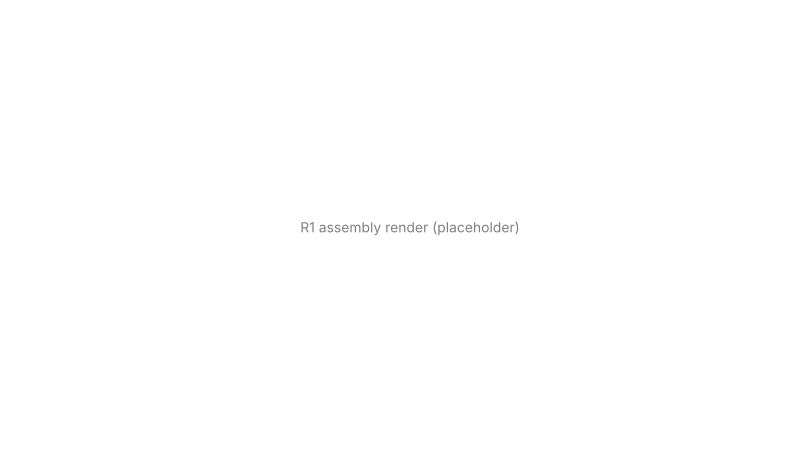
\includegraphics[width=0.85\linewidth]{R1_assembly}}
\begin{document}
\maketitle
\tableofcontents
% 01_introduction.tex
\chapter{Introduction}\label{sec:introduction}

% to be written (see docs/report_brief.md section 6)

% 02_requirements.tex
\chapter{Requirements}\label{sec:requirements}

% to be written (see docs/report_brief.md section 6)

% 03_sizing.tex
\chapter{Sizing from first principles}\label{sec:sizing}

% to be written (see docs/report_brief.md section 6)

% 04_loads.tex
\chapter{Loads}\label{sec:loads}

% to be written (see docs/report_brief.md section 6)

% 05_material.tex
\chapter{Material selection}\label{sec:material}

The material was chosen by an open trade study over the filaments the P1S can print, with the selected filament then assumed bought. The study follows the usual sequence of materials selection~\citep{ashby}: translate the design requirement into a merit index, remove the candidates that fail a hard limit, rank the rest by the index, and check the ranking against independent data before trusting it.

\section{Merit index for a stiffness-limited arm}\label{sec:material-index}

\Cref{sec:requirements,sec:loads} established that the frequency requirement, not strength, sizes the arms. The index follows from that, step by step.

\paragraph{What the arm must do.} With the motor and propeller as a tip mass $m_\text{tip}$ on a cantilever of free length $L$, the first bending frequency is
\begin{equation}
f = \frac{1}{2\pi}\sqrt{\frac{k}{m_\text{tip}}},
\end{equation}
so a frequency target fixes the tip stiffness:
\begin{equation}
k = (2\pi f)^2\, m_\text{tip}.
\end{equation}
The target and the tip mass are fixed, so $k$ is fixed, and every material must reach the same $k$.

\paragraph{How the arm makes that stiffness.} For a cantilever loaded at its tip,
\begin{equation}
k = \frac{3EI}{L^3},
\end{equation}
and for a rectangular section of width $b$ and height $h$,
\begin{equation}
I = \frac{bh^3}{12}.
\end{equation}
Substituting:
\begin{equation}
k = \frac{Ebh^3}{4L^3}.
\end{equation}

\paragraph{What is fixed and what is free.} The layout sets $L$. The width $b$ is held small, because every millimetre of width costs flight time through download (\cref{sec:sizing-width}). The height $h$ is free: it costs mass but no download. Each material therefore reaches the required $k$ with its own height. Solving for $h$:
\begin{equation}
h = \left(\frac{4kL^3}{Eb}\right)^{1/3}.
\end{equation}
With $k$, $L$ and $b$ fixed, $h$ grows as $E^{-1/3}$: a stiffer material needs a shallower arm, but only by the cube root.

\paragraph{What that costs in mass.} The arm's mass is
\begin{equation}
m = \rho\, b\, h\, L.
\end{equation}
Substituting $h$:
\begin{equation}
m = \rho\, b\, L \left(\frac{4kL^3}{Eb}\right)^{1/3}.
\end{equation}
Everything except $\rho$ and $E$ is the same for every material, so
\begin{equation}
m \propto \rho\, E^{-1/3}.
\end{equation}

\paragraph{The index.} The lightest arm comes from the material with the smallest $\rho E^{-1/3}$, which is the same as the largest
\begin{equation}
M = \frac{E^{1/3}}{\rho}.
\end{equation}
This is Ashby's index for a stiffness-limited beam whose width is fixed and whose height is free. Density counts in full, while modulus counts only through its cube root: a material twice as stiff makes the arm only 21\,\% shallower, because $2^{-1/3} = 0.79$. The index also depends on the constraint. A beam free to scale in both width and height would use $E^{1/2}/\rho$; holding the width small is what makes density dominate here. The index assumes a solid rectangular section with the frequency set by the tip mass. The optimised truss or ribbed section changes the absolute masses, but not the ranking between materials.

\section{Candidates and gates}\label{sec:material-gates}

The candidates are the eight filaments with complete technical data sheets from one manufacturer~\citep{bambu_tds}: PLA Basic, PLA-CF, PETG HF, PETG-CF, ASA, PET-CF, PAHT-CF and PPA-CF, all tested dry, at 100\,\% infill, with separate specimens printed in the layer plane ($xy$) and across the layers ($z$). TPU 95A HF was considered only for flexible parts.

Two gates remove candidates before any ranking.
\begin{itemize}
\item \textbf{Heat} (R5): heat deflection temperature at \SI{0.45}{MPa} of at least \SI{70}{\celsius}. The motors heat their mounts, and a frame that creeps at the motor pads loses its alignment. The motor-mount temperature after hard flights was not measured; \SI{60}{\celsius} is assumed, with a \SI{10}{\celsius} margin. The gate removes PLA (\SI{57}{\celsius}), PLA-CF (\SI{55}{\celsius}) and PETG HF (\SI{69}{\celsius}).
\item \textbf{Printability on the P1S}: PPA-CF needs a nozzle of 280 to \SI{310}{\celsius} against the printer's maximum of \SI{300}{\celsius}, and a heated chamber of 50 to \SI{80}{\celsius} that the P1S lacks. All carbon-fibre grades need a hardened steel nozzle.
\end{itemize}

\begin{figure}[htbp]
\centering
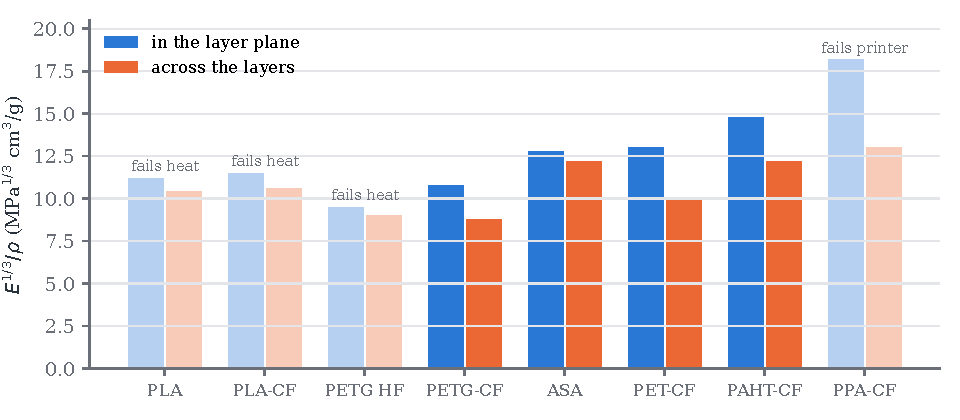
\includegraphics[width=0.95\linewidth]{plot_merit}
\caption{Frequency merit index of the candidates from manufacturer data, in the layer plane and across the layers. Pale bars fail a gate.}\label{fig:material-merit}
\end{figure}

\begin{table}[htbp]
\centering\small
\caption{Survivors of the gates, ranked by the merit index in the layer plane (manufacturer data). Arm mass is relative to a PLA arm of the same frequency.}\label{tab:material-ranking}
\begin{tabular}{@{}lccccc@{}}
\toprule
Material & Index $xy$ ($z$) & Arm mass & Strength $z$ (MPa) & Impact $z$ (kJ/m$^2$) & HDT (\si{\celsius})\\
\midrule
PAHT-CF & 14.8 (12.2) & 0.76 & 64 & 13.3 & 194\\
PET-CF & 13.0 (10.0) & 0.86 & 38 & 4.5 & 205 annealed\\
ASA & 12.8 (12.2) & 0.87 & 31 & 4.9 & 100\\
PETG-CF & 10.8 (8.8) & 1.04 & 38 & 10.7 & 74\\
\bottomrule
\end{tabular}
\end{table}

On manufacturer data PAHT-CF leads (\cref{fig:material-merit,tab:material-ranking}): the best index, the best across-layer strength and the best impact resistance. ASA has a low density and nearly isotropic stiffness but is brittle across layers and warps. PETG-CF is easy to print but marginal on the heat gate and the heaviest arm of the four.

\section{Anisotropy of printed material}\label{sec:material-anisotropy}

A printed part is a stack of layers, each made of extruded lines. Inside a line the polymer, and the short fibres it carries, are continuous and aligned with the print path; between lines and between layers the material is bonded only where the hot extrudate fused to the cold one beneath it. Across the layers ($z$) the data sheets give 46 to 87\,\% of the in-plane stiffness, 50 to 90\,\% of the in-plane strength, and only 10 to 52\,\% of the impact energy.

Coupon tests by the author on PLA (printed flat on a Bambu X1C, with rasters at \ang{0} and \ang{90} to the specimen axis) show the same pattern within a layer. Loading across the rasters lowered the modulus only slightly (2660 to \SI{3000}{MPa} against 2660 to \SI{3530}{MPa} along them) and the strength more (30 to \SI{43}{MPa} against 40 to \SI{59}{MPa}), and it cut the Charpy energy by roughly three to five times (0.08 to \SI{0.28}{J} against 0.36 to \SI{0.91}{J}). Impact across rasters and layers is the weakest property of every printed material. It steers the print orientation, which puts the bending stresses of the arms in the layer plane, and it is one reason the crash case is handled by a defined failure order instead of by strength.

\section{Independent data}\label{sec:material-independent}

Manufacturer data sheets may present their materials favourably, so the shortlist was checked against standardised independent tests of in-plane tensile strength and layer adhesion~\citep{mytechfun_siraya} (\cref{tab:material-independent}).

\begin{table}[htbp]
\centering\small
\caption{Manufacturer against independent strengths.}\label{tab:material-independent}
\begin{tabular}{@{}lcccc@{}}
\toprule
& \multicolumn{2}{c}{In the layer plane (MPa)} & \multicolumn{2}{c}{Across the layers (MPa)}\\
\cmidrule(lr){2-3}\cmidrule(l){4-5}
Material & sheet & independent & sheet & independent\\
\midrule
PAHT-CF (Bambu) & 88 & 67.4 & 64 & 20\\
PET-CF (Bambu) & 74 & 69 & 35 & 28.5\\
PET-CF (Siraya Fibreheart) & 74 & 64 & 35 & 28.1\\
\bottomrule
\end{tabular}
\end{table}

The across-layer strength of PAHT-CF on its data sheet, \SI{64}{MPa}, is three times the independent value of \SI{20}{MPa}. Both PET-CF grades agree with their sheets within about 20\,\%. PAHT-CF loses its main advantage, and it adds the drying a nylon needs (80\,\textdegree C for 8 to 12 hours) and the moisture sensitivity of its properties.

\section{Choice and design values}\label{sec:material-choice}

Siraya Tech Fibreheart PET-CF, a PET with 15\,\% short carbon fibre, printed unannealed, was chosen~\citep{siraya_petcf}. Its frequency index is 13.9 in the layer plane and 11.6 across the layers on its own data sheet. It passes the heat gate without annealing, with a heat deflection temperature of \SI{86.7}{\celsius} at \SI{0.45}{MPa}, so the distortion that annealing can cause is avoided. It costs \SI{40}{EUR/kg} against \SI{90}{EUR/kg} for the other PET-CF grade, and it prints at 280 to \SI{300}{\celsius} with a hardened nozzle. Its moduli were measured to ASTM D638 and the other grades' to ISO 527, so part of its 26 to 57\,\% higher moduli may come from the test method and the specimens.

The design values take the data-sheet moduli and the independent strengths, each multiplied by 0.85 for scatter and print settings (\cref{tab:material-design}).

\begin{table}[htbp]
\centering\small
\caption{Design values for Siraya Fibreheart PET-CF, unannealed.}\label{tab:material-design}
\begin{tabular}{@{}lccc@{}}
\toprule
Property & Source value & Design value ($\times 0.85$) & Allowable / 1.5\\
\midrule
$E_{xy}$ & \SI{5950}{MPa} & \SI{5058}{MPa} & \\
$E_z$ & \SI{3400}{MPa} & \SI{2890}{MPa} & \\
$S_{xy}$, tensile & \SI{64}{MPa} & \SI{54.4}{MPa} & \SI{36.3}{MPa}\\
$S_z$, layer adhesion & \SI{28.1}{MPa} & \SI{23.9}{MPa} & \SI{15.9}{MPa}\\
Density & \SI{1.30}{g/cm^3} & \SI{1.30}{g/cm^3} & \\
\bottomrule
\end{tabular}
\end{table}

No compressive or shear strengths exist for this material. Compression is taken equal to tension, which is conservative for fused-filament parts, where compressive strength is usually higher; shear between layers is checked against the layer adhesion strength, an assumption stated with the strength check.

\section{Material model}\label{sec:material-model}

Every part is printed with its layers in the global $xy$ plane, so the material is modelled as transversely isotropic with the build direction along $z$: one set of properties in the layer plane, another across it. Neither the data sheet nor the independent tests give Poisson's ratios or shear moduli. The model takes $\nu = 0.35$, inside the 0.2 to 0.4 reported for fused-filament materials, and derives the shear moduli from the isotropic relation in each plane:
\begin{equation}
G_{xy} = \frac{E_{xy}}{2(1+\nu)} = \frac{5058}{2.7} = \SI{1873}{MPa}, \qquad G_{xz} = G_{yz} = \frac{E_z}{2(1+\nu)} = \frac{2890}{2.7} = \SI{1070}{MPa}.
\end{equation}
The error this assumption can cause is small. A Timoshenko beam model of the arm attributes 13\,\% of its tip deflection to shear, and changing $G$ from 700 to \SI{1500}{MPa} moves its first frequency from 665 to \SI{700}{Hz}, $-3$ to $+2$\,\% around the \SI{687}{Hz} of the nominal value, well inside the margin of the frequency goal.

\section{Flexible parts and cost}\label{sec:material-cost}

The retainers that hold the receiver, the GPS and the antenna, and the skid on the floor of the body, are printed in TPU 95A HF, a thermoplastic polyurethane whose flexibility allows snap fits and press fits, and whose impact and abrasion resistance suits a sacrificial landing surface. They are not part of the optimised structure.

At 20 to \SI{100}{EUR/kg}, a frame of about \SI{60}{g} costs roughly 1 to \SI{6}{EUR} of filament for any candidate, against \SI{37.91}{EUR} for the reference frame. Cost does not discriminate between the candidates; the frame meets R9 whichever filament is chosen.

% 06_architecture.tex
\chapter{Architecture, joint and design space}\label{sec:architecture}

% to be written (see docs/report_brief.md section 6)

% 07_topopt_theory.tex
\chapter{Topology optimisation theory}\label{sec:topopt_theory}

% to be written (see docs/report_brief.md section 6)

% 08_optimisation_model.tex
\chapter{Optimisation model and runs}\label{sec:optimisation_model}

% to be written (see docs/report_brief.md section 6)

% 09_iterations.tex
\chapter{Design iterations driven by verification}\label{sec:iterations}

The design space went through four iterations. None was planned: each was forced by a check on a result that the optimiser reported as a success. This chapter follows them in order, because each one added a rule to the design space that applies to any printed part optimised this way. \Cref{sec:optimisation_model} describes the model and the runs; \cref{sec:verification} the thresholded checks and the print geometry in full.

\begin{table}[htbp]
\centering\small
\caption{Design-space iterations: what each check found and what changed.}\label{tab:iter-summary}
\begin{tabularx}{\linewidth}{@{}lXX@{}}
\toprule
Result checked & Finding & Change for the next iteration, and rule\\
\midrule
Iteration 1 & structure meets every requirement at \SI{76.8}{g}, but no component can be installed & tub and lid; insertion, tool and cable paths as keep-outs\\
Iteration 2 & the receiver-antenna boss becomes a loose island & fixed antenna spine; every fixed region is kept by a load, a mass or a fixed link\\
Iteration 2, per part & a lid boss on the keel is held only by the lid; the GPS deck hangs from the lid & GPS deck moved to the tub, keel boss deleted; the rule applies within each part\\
Iteration 4 & GPS deck connected but carried by grey material; first mode \SI{146.8}{Hz} & keel zone cleaned, hand-drawn keels; connectivity is not stiffness\\
\bottomrule
\end{tabularx}
\end{table}

\section{Iteration 1: a structure that cannot be built}\label{sec:iter-1}

The first design space defined where every component sits: the battery plate as a fixed part of a one-piece centre body, voids above the flight controller for the receiver and the capacitor, a USB window, wire channels at the corners, a strap tunnel, and the rear keel under the GPS pad as design space. The production run on it converged to a feasible design after 28 cycles and was stopped after 40, with the frequency constraint and three of the four compliance caps active.

\subsection{The structure passed}

Thresholded at iso levels 0.5 and 0.3, both cuts met every requirement and were stiffer than the optimiser predicted (\cref{tab:iter-1}). The solid elements kept are fully stiff, while the optimiser counted grey ones at less than their share of the mass (\cref{tab:to-interp}), so grey material had not been over-credited. The design space was well separated: 47\,\% of the design elements below 0.3, 5\,\% between 0.3 and 0.5, and 48\,\% at or above 0.5. Cut at 0.4, smoothed and restored with the exact fixed regions, the frame weighed \SI{76.8}{g}: a body of \SI{45.58}{g} and four arms of \SI{7.81}{g}.

\begin{table}[htbp]
\centering\small
\caption{First design space, last cycle: optimiser against the thresholded bodies.}\label{tab:iter-1}
\begin{tabular}{@{}lrrr@{}}
\toprule
Model & First elastic mode & Modes 8 to 12 (Hz) & Compliance / cap\\
\midrule
Optimiser (grey) & \SI{417.8}{Hz} & 419.7 to 521.2 & 0.98 to 1.00\\
Thresholded, iso 0.5 & \SI{438.3}{Hz} & 446.1 to 547.4 & 0.86 to 0.93\\
Thresholded, iso 0.3 & \SI{449.5}{Hz} & 462.5 to 574.9 & 0.76 to 0.84\\
\bottomrule
\end{tabular}
\end{table}

\subsection{A check that stopped the wrong runs}

The runs on this design space also corrected a check. Spurious local modes (\cref{sec:to-spurious}) were guarded against by a rule that flagged any mode whose largest motion sat mostly in elements below density 0.3. It stopped a coarse run at cycle 10 and would have stopped the production run at cycle 20. The flagged modes were the arm bending modes: smooth, with their maxima at the motor seats, frequencies continuous with the history, and peak regions of thousands of nodes at mean densities of 0.2 to 0.45. The rule detected grey material in a mode, which is where the optimiser had made thin walls at the arm tips, not a spurious mode. The thresholded model, which measures the printable part directly, passed. From then on the mode check was a reported diagnostic, and the thresholded model at the print level became the acceptance test.

\subsection{The assembly failed}

Looked at as a part to build, the result was useless. The flight-controller bay was closed on every side: the only openings were the USB window, the strap tunnel, \SI{4}{mm} lead passages at the foot of each wall and slits of 1 to \SI{3}{mm} at the wall corners, and the roof was the fixed battery plate over an optimised ceiling. The board could not enter from any side, because 607 to \SI{861}{mm^3} of design material blocked each direction. The screw holes of its bosses were blind, with no screwdriver line, and nothing passed the battery lead, the GPS cable or the antenna.

The cause was in the design space, not in the optimiser. The design space said where each component sits but not how it gets there, and the optimiser filled every path, as it should: material that helps the stiffness and costs nothing under the constraints is material it keeps.

\subsection{Iteration 2: tub, lid and assembly paths}

The second design space was drawn around an assembly sequence (\cref{sec:arch-designspace}). The centre body became an open tub with a removable lid carrying the battery plate and, at this stage, the GPS deck. Every component received an insertion path, a tool path and a cable path as keep-outs, each checked by a sweep in an automated clash test. The board received \SI{4}{mm} of clearance on every side, so the body grew to $46\times46$\,mm and the corners moved out by \SI{3}{mm}. Each component got a designed seat and a retainer, with no glue or tape.

The lid created a new question: how is it connected to the tub? A reference analysis on the solid design space answered it. Tied at its screw bosses alone, the lid let a plate mode carrying the battery fall to \SI{405.1}{Hz} and pulled an arm saddle mode to \SI{389.8}{Hz}, below the goal. Tied over its whole seat on the tub rim, the same modes moved to 449.7 to \SI{654.6}{Hz}. In every static load case the battery's inertia presses the lid onto the rim and the screws preload it, so full contact is the real state as long as the seat is flat. The model ties the lid over the whole seat, and the printed lid underside and tub rim carry a flatness requirement of \SI{0.1}{mm}, checked with a feeler gauge before assembly.

The production run on iteration 2, thresholded at 0.4 with the seat tied, passed with a first mode of \SI{426.8}{Hz}. With the lid held at the five screw bosses only, the same body failed at \SI{192.1}{Hz}, a GPS deck mode below even the \SI{290}{Hz} minimum. The design relies on the seat contact, which the flatness requirement protects.

\section{Iterations 2 to 4: islands}\label{sec:iter-islands}

\subsection{An island at the antenna mount}

In iteration 2 the receiver antenna was held by a TPU clip screwed to a small fixed boss under the rear keel. In the optimisation that boss touched only design material and carried no load and no mass, because the antenna's mass was lumped with the flight controller. Nothing required a load path to it, so the optimiser removed the keel material around it. Thresholded, the boss was a loose part of \SI{0.15}{g} with six rigid-body modes between 45 and \SI{200}{Hz} on near-empty material.

Iteration 3 routed the antenna cable through a fixed sleeve, \SI{1.5}{mm} thick, from the bay into the keel, ending in a pad under the keel with an insert boss for the holder and a locating hole for its peg; a fixed web continues the sleeve up the rear wall into a lid boss. The chain from antenna to lid boss is fixed throughout, so the mount cannot be cut loose, and the antenna, holder, screw and insert (\SI{2.24}{g}) now act as a point mass on the pad. The antenna itself became a straight T (its moulded junction cannot bend), hanging vertically under the cable exit so the coax enters the stem without a bend, routed through one bend of radius \SI{7}{mm}, more than the six cable diameters the connector maker recommends. The spine added \SI{1.54}{g} of fixed material and passed 35 geometric checks, among them \SI{5.32}{mm} from the antenna legs to the rear arms.

The finding became a design-space rule: every fixed region either touches other fixed material or carries a load, a tie or a mass that needs a solid path. It is checked at export and after every thresholding by an island check.

\subsection{An island held by the other part}

The rule was then applied part by part. A lid boss on the keel carried the tie to the lid, and in the assembled model the lid held it. Checked on the tub alone, the boss was an island of \SI{141.4}{mm^3}, \SI{3.78}{mm} from the main tub at iso 0.4 and joined only by a chain of single elements between 0.3 and 0.4; all tub material behind it had been removed. The optimiser had used the lid as the boss's support. The GPS deck, then part of the lid, also hung from the lid as a cantilever.

Iteration 4 moved the GPS deck, with its pocket rim and cap bosses, from the lid to the tub, on top of the keel. The lid now ends at the battery plate with a \SI{0.5}{mm} gap to the deck and no tie between them, and the keel boss was deleted: the lid is clamped by the four wall bosses. Each lid screw pad is joined to the plate frame by a fixed link \SI{4.5}{mm} wide, so the lid's fixed region is one cell. The GPS mass now needs a load path through the tub, and the lid no longer supports anything it does not own. The rule was restated per part: each fixed region is kept by a load, a mass or a fixed link within its own part. The seat area shrank from 625.98 to \SI{363.23}{mm^2} on the tub side, and the full-density mass fell by \SI{0.09}{g}.

\section{Iteration 4: connected, but grey}\label{sec:iter-grey}

The production run on the fourth design space reduced the design volume by 55.4\,\% in 28 cycles (\cref{sec:optimisation_model}). The island check passed for every part at iso 0.3 and 0.4: the four wall bosses, the GPS deck and the lid were all connected. The thresholded model failed anyway. Its first elastic mode was a GPS deck mode at \SI{146.8}{Hz}, and the landing compliance exceeded its cap by 20\,\%. In the optimisation the deck had been carried at \SI{461.7}{Hz} by a wide block of keel material with densities mostly below 0.15. Such material is penalised in stiffness but still contributes, and no threshold keeps it: thresholded at any level from 0.3 to 0.5, the deck hung from two thin straps at its front.

\subsection{Five supports on the same density field}

Five supports were tested on the saved density field of the last cycle without a new optimisation, by forcing elements solid or empty inside a defined shape (\cref{tab:iter-keels,fig:iter-keels}).

\begin{table}[htbp]
\centering\small
\caption{Supports for the GPS deck, each checked as a thresholded model on the density field of the production run.}\label{tab:iter-keels}
\begin{tabular}{@{}lcccc@{}}
\toprule
Support & Model mass & First elastic mode & LC3a compliance / cap & Result\\
\midrule
As optimised, iso 0.4 & \SI{281.3}{g} & \SI{146.8}{Hz} & 1.20 & fail\\
As optimised, iso 0.3 & & \SI{162.3}{Hz} & & fail\\
Local iso 0.15 in the keel & \SI{281.5}{g} & \SI{380.6}{Hz} & 0.99 & fail\\
Two full side webs forced solid & \SI{283.4}{g} & \SI{430.7}{Hz} & 0.93 & pass\\
Keel zone cleaned, web B only & \SI{281.1}{g} & \SI{7.8}{Hz} & 28.05 & fail\\
Keel zone cleaned, keels A & \SI{282.2}{g} & \SI{420.7}{Hz} & 0.95 & pass\\
Keel zone cleaned, keels A and web B & \SI{282.3}{g} & \SI{428.4}{Hz} & 0.94 & pass\\
\bottomrule
\end{tabular}
\end{table}

\begin{figure}[htbp]
\centering
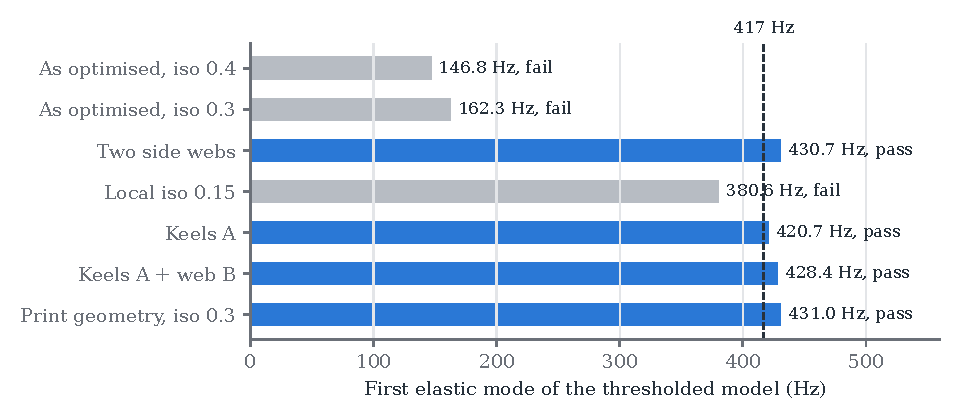
\includegraphics[width=0.95\linewidth]{plot_keels}
\caption{First elastic mode of each support variant against the \SI{417}{Hz} goal.}\label{fig:iter-keels}
\end{figure}

Lowering the threshold locally to 0.15 failed: the optimiser had not formed a structure in the keel at all, only a diffuse field. Two full-depth side webs passed, at \SI{2.11}{g} of forced material. The adopted design cleans the keel zone of all design material and adds two shapes drawn by hand, closer to what the optimiser had been building.
\begin{itemize}
\item \textbf{Keels A}: twin tapered keels hanging from the deck underside, mirrored in $y$, between $|y| = 4.6$ and the deck edge or the propeller sweep plus \SI{3}{mm}, flaring into the rear wall. Their depth grows towards the wall, where their bending moment is largest:
\begin{equation}
z_\text{bot}(x) = 21.5 - 11.5\left(0.6\,t + 0.4\,t^2\right), \qquad t = \frac{x + 50}{28},
\end{equation}
zero depth at $x = -50$ and \SI{11.5}{mm} deep at the wall.
\item \textbf{Web B}: a web \SI{2}{mm} thick under the antenna sleeve, from the sleeve to the rear wall, its lower edge one straight line from \SI{1}{mm} below the sleeve to the wall face at $z = -2.0$, \SI{1}{mm} above the opening for the motor leads.
\end{itemize}
Web B alone does not reach the deck and fails, but it braces the antenna spine: with it, mode 12 rises from 458.5 to \SI{529.6}{Hz}. Keels A and web B meet every requirement with \SI{1.1}{g} less than the side webs at the same margins, and the final print geometry with the exact solids reaches \SI{431.0}{Hz} (\cref{sec:verification}).

\begin{figure}[htbp]
\centering
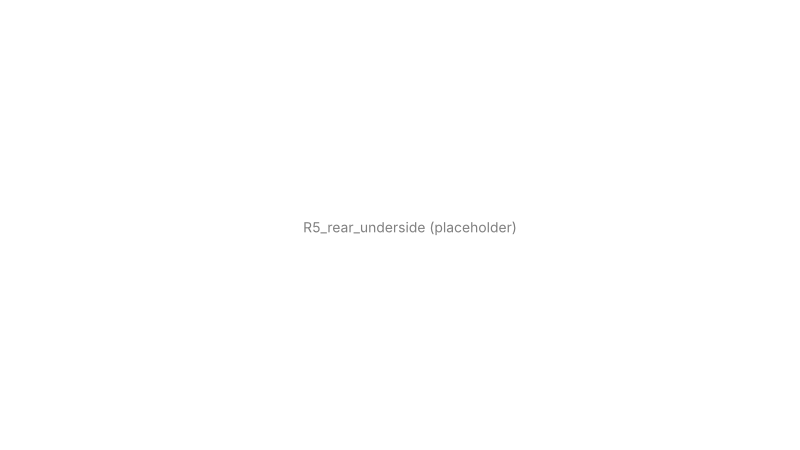
\includegraphics[width=0.85\linewidth]{R5_rear_underside}
\caption{Rear underside of the printed tub: twin keels under the GPS deck, the web under the antenna sleeve, the antenna pad and holder.}\label{fig:iter-rear}
\end{figure}

\subsection{Exact solids}

The keels were then drawn as exact solids for printing, from the same definitions (\cref{fig:iter-rear}). They differ from the element shapes of the check only where printability or mesh quality required it, and they hold more material, except for two pieces thinner than one element: each end stops with a face at least \SI{1}{mm} deep instead of a feather edge, every piece is at least \SI{1.2}{mm} wide, and the keels clip the cable channels and the propeller sweep exactly. Keels A are two solids of \SI{1315.1}{mm^3} (\SI{1.71}{g}) against \SI{1149.4}{mm^3} in the element shape, and web B is \SI{119.7}{mm^3} (\SI{0.16}{g}).

\section{Rules}\label{sec:iter-rules}

The four iterations left four rules, each stated so that it can be checked by a script.
\begin{enumerate}
\item \textbf{Assembly}: every component has an insertion path, a tool path and a cable path as keep-outs, checked by a sweep in the clash test.
\item \textbf{Connectivity}: every fixed region is kept by a load, a mass or a fixed link within its own part, checked at export and by an island check per part after every thresholding.
\item \textbf{Stiffness}: a fixed region that carries a mass or a load gets either a fixed load path to the main structure or a design corridor narrow enough that the optimiser must form a defined member in it. The thresholded model, not the island check, decides.
\item \textbf{Acceptance}: the result is accepted on the thresholded model at the print level, with every frequency and compliance requirement, not on the optimiser's grey model or on a mode diagnostic.
\end{enumerate}
The fourth design space would have revealed its grey keel within hours, not after a production run of seven and a half hours, if a coarse rehearsal had been thresholded and checked on its saved cycles first.

% 10_verification.tex
\chapter{Thresholded verification and print geometry}\label{sec:verification}

% to be written (see docs/report_brief.md section 6)

% 11_strength.tex
\chapter{Strength and capacity}\label{sec:strength}

% to be written (see docs/report_brief.md section 6)

% 11b_capacity.tex: capacity reasoning, follows the strength sections of chapter 11
\section{Capacity and failure order}\label{sec:capacity}\label{sec:strength-capacity}

Capacity design (\cref{sec:loads-capacity}) asks that the arm fail before the joint and the centre body, with a margin of 1.5 on the failure force. The check is geometric: it compares the strength of each arm section with the strength of the joint, both for the same load, a vertical force at the arm tip.

\subsection{Failure force of an arm section}

A vertical force $F$ at the motor axis, at a distance $u_m = \SI{74.25}{mm}$ from the frame centre along the arm, bends every section of the arm at a position $u$ with a lever $u_m - u$:
\begin{equation}
M(u) = F\,(u_m - u).
\end{equation}
A section of elastic section modulus $Z = I/c_\text{max}$ (second moment of area about its horizontal centroidal axis, divided by the largest vertical distance from that axis) reaches the in-plane strength when $M = S_{xy} Z$. The tip force that fails the section at $u$ is therefore
\begin{equation}
F_\text{arm}(u) = \frac{S_{xy}\, Z(u)}{u_m - u}.
\end{equation}
The arm fails at the section where $Z/(u_m - u)$ is smallest, which is not necessarily where $Z$ is smallest: a slim section close to the tip has a short lever.

\subsection{Failure force of the joint}

The joint carries a vertical moment of $M_j = \SI{21216}{N.mm}$ by bearing at its two bolts (\cref{sec:arch-joint}). Its own lever to the motor axis is $u_m - u_j$, with the bolt line at $u_j = \SI{37.24}{mm}$, so the tip force that fails it is
\begin{equation}
F_\text{joint} = \frac{M_j}{u_m - u_j} = \frac{21216}{37.00} = \SI{573}{N}.
\end{equation}

\subsection{Why the planning rule was not conservative}

At the planning stage the requirement was written as a limit on the section modulus at the fork exit, $Z \leq M_j/(1.5\,S_{xy}) = \SI{260}{mm^3}$. That rule compares moments at the same section, as if arm and joint had the same lever. They do not: the fork exit is outboard of the bolt line, so for the same tip force it carries a smaller moment. Requiring the arm's failure force at the fork exit ($u = \SI{43.74}{mm}$) to be at most $F_\text{joint}/1.5$ gives
\begin{equation}
\frac{S_{xy}\, Z}{u_m - u} \leq \frac{1}{1.5}\,\frac{M_j}{u_m - u_j} \quad\Rightarrow\quad Z \leq 260\,\frac{u_m - u}{u_m - u_j} = 260 \times \frac{30.51}{37.01} = \SI{214}{mm^3}.
\end{equation}
The moment rule allowed a section 21\,\% stronger than the force rule. More important, the fork exit is not where the printed arm is weakest.

\subsection{The printed arm}

Sections normal to the arm axis were cut from the printed geometry of one arm, and $Z$ computed from the exact section polygons, with the method validated on bars of known section. At the fork exit $Z = \SI{815.6}{mm^3}$, three times the planning limit, and $Z$ falls steadily outwards to \SI{131.9}{mm^3} at $u = 61$ to \SI{62}{mm}, just inside the motor pad. Divided by the lever (\cref{tab:cap-lever}), the minimum of $Z/(u_m - u)$ is \SI{9.96}{mm^2} at that slim section, with a lever of \SI{13.25}{mm}.

\begin{table}[htbp]
\centering\small
\caption{Section modulus of the printed arm divided by its lever to the motor axis.}\label{tab:cap-lever}
\begin{tabular}{@{}lrrrrrrrrr@{}}
\toprule
$u$ (mm) & 45 & 50 & 55 & 58 & 60 & 61 & 62 & 66 & 70\\
\midrule
$Z$ (mm$^3$) & 584.2 & 530.4 & 381.4 & 210.5 & 155.3 & 131.9 & 122.0 & 145.3 & 138.3\\
$Z/(u_m - u)$ (mm$^2$) & 19.98 & 21.88 & 19.82 & 12.96 & 10.90 & 9.96 & 9.96 & 17.62 & 32.58\\
\bottomrule
\end{tabular}
\end{table}

The slim section fails at $F_\text{arm} = 54.4 \times 9.96 = \SI{542}{N}$, and the ratio of the two failure forces is
\begin{equation}
\frac{F_\text{arm}}{F_\text{joint}} = \frac{S_{xy}\, Z/(u_m - u)}{M_j/(u_m - u_j)} = \frac{54.4 \times 9.96 \times 37.00}{21216} = 0.95.
\end{equation}
\begin{figure}[htbp]
\centering
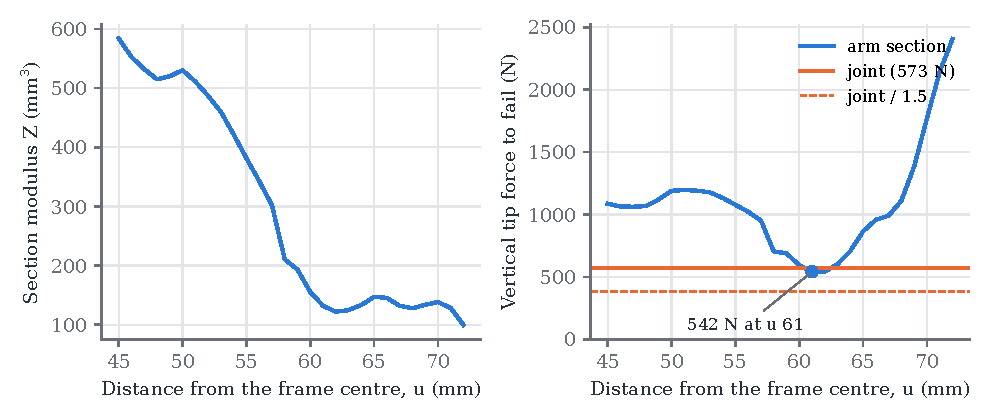
\includegraphics[width=\linewidth]{plot_capacity}
\caption{Left: section modulus of the printed arm for vertical bending along its length. Right: the vertical tip force that fails each section, against the joint capacity. The slim section near the motor pad fails at \SI{542}{N}, the joint at \SI{573}{N}.}\label{fig:cap-capacity}
\end{figure}

By this estimate (\cref{fig:cap-capacity}) the arm is marginally the weaker element, but 0.95 lies inside the scatter of both estimates: the joint's bearing allowable is assumed equal to $S_{xy}$, and the arm is taken to fail at first-fibre stress. Which one fails in a vertical overload is not controlled. A margin of 1.5 needs a ratio of 0.67 or less. The vertical failure order (R4) is not met.

Sideways the order holds with a factor of 8.5, because the fork resists in-plane bending with its full width. The fin root on the tub keeps a section modulus of \SI{957.2}{mm^3} where it leaves the body corner and at least \SI{792.4}{mm^3} along its length, against the \SI{390}{mm^3} it needs, so a joint failure would be in bearing at the bolt holes, not across the fin root.

\subsection{Why, from first principles}

Two facts combine. First, the frequency optimisation puts arm depth where the bending moment of the arm modes is largest, at the root and the joint, and removes material near the tip, where it moves without bending (\cref{sec:to-frequency}). The section that comes out weakest under a tip force is therefore the one near the motor, and the optimiser has no reason to make it stronger: a stiffness or frequency requirement says nothing about the order in which parts fail. Second, the joint was sized as balanced: the fin and the two prongs carry the same bearing force when $t_\text{fin} = 2t_\text{prong}$, so inside the joint neither the tub nor the arm is the weaker element. Capacity design has to be imposed on the joint and on the arm explicitly; it does not emerge from an optimisation for stiffness.

\subsection{Redesign}

The redesign makes the arm part, which is replaceable, the fuse. Either option needs a new thresholded frequency check, because the frequency margin of the print geometry is 3.4\,\% ($431.0/417 = 1.034$).
\begin{enumerate}
\item[(A)] \textbf{Prongs as the fuse.} Unbalance the joint so the prongs, which belong to the arm, are 1.5 times weaker in bearing than the fin, which belongs to the tub. With the fin at \SI{10}{mm}, prongs of \SI{3.3}{mm} give
\begin{equation}
\frac{F_{b,\text{fin}}}{F_{b,\text{prongs}}} = \frac{54.4 \times 3 \times 10}{2 \times 54.4 \times 3 \times 3.3} = \frac{1632}{1077} = 1.52.
\end{equation}
In a vertical overload the bolts then tear out of the prongs, and the tub is untouched.
\item[(B)] \textbf{A defined fuse section near the motor.} Keep the joint and limit the slim section so the ratio reaches 0.67:
\begin{equation}
Z \leq 0.67 \times \frac{M_j}{S_{xy}\,(u_m - u_j)}\,(u_m - u) = 0.67 \times \frac{21216}{54.4 \times 37.00} \times 13.25 \approx \SI{90}{mm^3},
\end{equation}
against \SI{131.9}{mm^3} now. The arm then breaks next to the motor pad.
\end{enumerate}
Option A changes only the fixed geometry of the joint, which the optimiser does not touch, so it keeps the optimised arm. Option B thins the section where the arm's bending stiffness matters least for the umbrella mode, but it lowers the strength margin of every load case at that section.

% 12_retainers.tex
\chapter{Retainers and integration}\label{sec:retainers}

% to be written (see docs/report_brief.md section 6)

% 13_results.tex
\chapter{Results, limitations and future work}\label{sec:results}

% to be written (see docs/report_brief.md section 6)

\appendix
% A_logs.tex
\chapter{Decision log, numbers and assumptions}\label{sec:logs}

\section{Decision log}\label{sec:logs-decisions}

The decisions that shaped the frame, in the order they were taken, numbered for this report. Each records what was decided, the options weighed and the reason.

\small
\begin{xltabular}{\linewidth}{@{}r>{\raggedright\arraybackslash}p{0.36\linewidth}X@{}}
\toprule
No. & Decision & Options and reason\\
\midrule
\endfirsthead
\toprule
No. & Decision & Options and reason\\
\midrule
\endhead
\bottomrule
\endfoot
1 & Baseline battery: four-cell \SI{850}{mAh}, \SI{100}{g} & The pack that is bought and flown; a lighter high-voltage \SI{1100}{mAh} pack is reported for information only\\
2 & Printer: Bambu Lab P1S & The available printer; it sets the printability gate of the material study\\
3 & Material chosen by an open trade study over all candidate filaments & Shows the selection logic in full; the chosen filament is assumed bought\\
4 & Component masses from manufacturers' data & Faster than weighing; labelled as data-sheet values in the budget\\
5 & Commercial carbon frame as a reference, not a target & Printed thermoplastic cannot match continuous-fibre plate on specific stiffness; the comparison quantifies the gap and the cost saving\\
6 & Physical testing reduced to a test plan & Effort goes to design, optimisation and analysis\\
7 & Mass requirement: take-off mass below \SI{250}{g} with GPS, without payload; frame budget \SI{61.4}{g} & EU open category A1; its \SI{19}{m/s} speed limit is acknowledged and left to the flight firmware\\
8 & Factor of safety 1.5 on printed allowables & Conventional aircraft ultimate factor\\
9 & Flight time and thrust-to-weight are outputs, not requirements & Set by the components; the frame acts on them only through mass, which the mass requirement controls; ten grams cost less flight time than the model's uncertainty\\
10 & Camera payload excluded from the baseline & Keeps the work focused on the frame; next step\\
11 & Hover power model $a n^3 + b n$, with $a n^3 + c$ as the conservative bound & Only these two pass the efficiency-trend test; the chosen one has physical terms and the better fit\\
12 & Arm root moment from the full thrust, without the motor's inertia relief & The relief disappears in asymmetric manoeuvres and when the aircraft is restrained\\
13 & Motor thermal check by rating comparison; heat deflection gate of \SI{70}{\celsius} on the material & Hover draws about 7\,\% of the motor's rated peak; the frame-relevant question is the mount temperature against the material\\
14 & True X layout, wheelbase \SI{148.5}{mm}, propeller gap \SI{16.1}{mm} & Shortest arms for a given gap; four identical arms; the wheelbase grew from \SI{140}{mm} to give the flight controller assembly room without changing the arms\\
15 & Battery on top, on a raised plate above the blade tips & Centre of gravity near the rotor plane, punch-out load into the plate in compression, frame bottom free for landings; roll inertia within 4\,\% of a bottom mount\\
16 & Structural direction: printed centre body topology-optimised, tall narrow tapered arms & Puts printing where it is strong, in three-dimensional nodes and deep sections; narrow arms keep the download low\\
17 & No ring between the motors & Adds no stiffness to the umbrella mode and lowers it; an inner ring doubles the download per millimetre; an outer guard weighs 20 to \SI{30}{g}\\
18 & Body floor level with the arm bottoms; strap across the battery width through a tunnel & The root moment passes into the body over the full arm depth; the strap stays out of the propeller clearance\\
19 & Voids for components and wiring, then insertion, tool and cable paths for every component & Without them the optimiser fills the space and the paths; checked by sweeps in a clash test\\
20 & Crash case by capacity design: arm the weakest link, joint and body sized for 1.5 times its failure load & A crash speed gives arbitrary forces; capacity design fixes where failure occurs\\
21 & First free-free elastic mode at least \SI{290}{Hz}, goal \SI{417}{Hz} & The goal halves the response at hover 1P and leaves margin for modelling error, at about twice the stiffness of the minimum\\
22 & Landing: firm landing as a design case, motor cut as a survivability check; thin sacrificial skid & Ground pressure is negligible; the deceleration of each mass loads the structure\\
23 & Arm underside rising to \SI{9}{mm} of ground clearance at the tip & The body is the landing point; about \ang{12} of tilt before a motor touches\\
24 & Material: Siraya Fibreheart PET-CF, unannealed; design values with a 0.85 knockdown & Best cost and performance after independent tests removed the leading candidate's across-layer advantage; passes the heat gate unannealed\\
25 & Skid: TPU, sliding into a dovetail in the floor, no screws & Landing presses it on, scraping acts along the dovetail; replaceable without tools\\
26 & Optimiser: Abaqus with Tosca Structure & Documented frequency constraint with mode handling; the same model serves the strength check\\
27 & Free-flying cases with inertia relief and 3-2-1 supports & A clamp carries load that does not exist in flight and attracts material; determinate supports carry nothing\\
28 & Formulation: minimum volume, modes 7 to 12 at least \SI{417}{Hz}, one compliance cap per case & States the real goal; one limit per case removes the weighting problem\\
29 & The printed part is the smoothed optimised surface, with exact fixed regions restored & A manual rebuild loses the load paths and is not more printable\\
30 & Transversely isotropic material, build direction $z$ & Arms bend in the layer plane, walls and joints load across it\\
31 & Arm envelope at the full depth the propellers allow & For the same frequency the deep profile needs half the arm mass\\
32 & Fin-and-fork joint with two horizontal M3 bolts & Fits beside the flight controller, continues the deep arm into the body, bolts in shear, inserts along the layers\\
33 & Joint detail rules: load through bolts and clamped faces only, gaps sized by function & Defines the load path; nose and fillet gaps never close under tolerances\\
34 & Joint sizing: fin \SI{10}{mm}, prongs \SI{5}{mm}, bolts \SI{13}{mm} apart & Fin and prongs balanced in bearing; capacity \SI{21216}{N.mm}\\
35 & Failure order and fin-root strength checked on the optimised geometry & The optimised arm is unknown until the optimisation ends\\
36 & Interfaces fixed only where they function: plate frame and strap band, motor screw bosses and contact ring & Material at the arm tip costs frequency most\\
37 & Joint bosses as through-cylinders extended to the arm top & Removes slivers that the mesher cannot fill; one split rule for the whole model\\
38 & Minimum member size \SI{2.5}{mm}, mesh \SI{1.0}{mm} & Six extrusion lines; the restriction needs more than twice the element size\\
39 & Identical arms enforced by a cyclic symmetry restriction & One spare fits all four positions; the body stays free because the loads are not symmetric\\
40 & Runs staged: reference, smoke test, coarse run, production & Each stage removes one risk before the expensive run\\
41 & Caps at twice the solid compliance on the same mesh & A finer mesh is more flexible; caps from a coarser mesh would be too tight\\
42 & Mass requirement not met at \SI{417}{Hz}; accepted; frequency sweep deferred & The design space needs about three times the mass allowance at this frequency\\
43 & Acceptance on the thresholded model at the print level; mode check as a diagnostic & The mode check detected grey material, not spurious modes, and stopped runs that passed once thresholded\\
44 & Open tub with a removable lid & A vertical insertion path and straight tool paths; windows large enough for the board would remove a wall\\
45 & Components held by designed seats and retainers, no glue or tape & Maintainable and repeatable assembly\\
46 & Flight controller on through-bosses, screws from below, nuts from above & Blind bosses had no tool path\\
47 & Lid tied over its whole seat; flatness \SI{0.1}{mm} required & With bosses only a lid mode fell below the goal; the battery and the screws press the lid on the rim in every load case\\
48 & Antenna spine and the connectivity rule & A boss touching only design material was cut loose\\
49 & GPS deck on the tub, keel boss deleted & The lid had been holding tub material; each part now carries its own\\
50 & Keel zone cleaned, hand-drawn keels and web; the stiffness rule & The deck was connected but carried by grey material that no threshold keeps\\
51 & Print at iso 0.3, tub floor-down & Thicker thin members for \SI{3.57}{g}; layers in the $xy$ plane\\
52 & Vertical failure order reported as not met; redesign by a prong fuse or a fuse section & Arm and joint fail at about the same force; no time for a geometry change and a new check\\
\end{xltabular}
\normalsize

\section{Numbers}\label{sec:logs-numbers}

The numbers quoted in this report, with their source.

\small
\begin{xltabular}{\linewidth}{@{}>{\raggedright\arraybackslash}p{0.48\linewidth}>{\raggedright\arraybackslash}p{0.22\linewidth}X@{}}
\toprule
Quantity & Value & Method\\
\midrule
\endfirsthead
\toprule
Quantity & Value & Method\\
\midrule
\endhead
\bottomrule
\endfoot
Fixed component mass & \SI{168.6}{g} & data sheets\\
Thrust constant; thrust coefficient & \SI{3.088e-7}{g/RPM^2}; 0.1425 & least squares, bench data\\
Download fraction, \SI{8}{mm} arm & 3.0\,\% (2.2 to 3.9) & actuator disc and plate drag\\
Hover thrust per motor; speed & \SI{64.4}{g}; 14,440\,RPM & at \SI{250}{g}\\
Hover 1P and 3P; full-throttle 1P and 3P & 241, \SI{722}{Hz}; 679, \SI{2038}{Hz} & speed / 60\\
Hover power per motor; aircraft & \SI{18.3}{W}; \SI{74}{W}, \SI{5.0}{A} & fitted model\\
Hover flight time & \SI{8.2}{min} (6.6 to 9.0) & usable energy over power\\
Cost of one gram; of \SI{1}{mm} of arm width & \SI{-0.036}{min}; \SI{-0.035}{min} & sensitivity\\
Maximum thrust; motor torque; load factor & \SI{5.04}{N}; \SI{0.040}{N.m}; 8.2 & bench, torque constant\\
Thrust-to-weight with battery sag & 5.4 to 7.3 & coupled voltage and current\\
Top speed; kinetic energy & \SI{30}{m/s} (27 to 36); \SI{114}{J} & tilt balance\\
Landing load factors & 23 (firm), 200 (motor cut) & spring energy balance\\
Design values, PET-CF & $E$ 5058 / \SI{2890}{MPa}; $S$ 54.4 / \SI{23.9}{MPa} & data sheet and independent tests $\times$ 0.85\\
Solid arm corridor, first frequency & 736 / \SI{557}{Hz} & beam model, clamped\\
Joint capacity & \SI{1632}{N} per bolt; \SI{21216}{N.mm} & bearing at $S_{xy}$\\
Final design space: tub, lid, arm (design / fixed) & 39,538.5 / 12,796.3; 2,357.0 / 3,417.1; 8,036.9 / 2,933.5\,mm$^3$ & generator\\
Point masses in the model & \SI{199.58}{g} & components, hardware, retainers\\
Production run & 28 cycles, 7\,h\,34\,min; volume $-55.4$\,\% & 765,252 C3D10 elements\\
Print-set masses & tub 47.21, lid 6.61, arm 8.85, frame \SI{89.22}{g} & iso 0.3, restored\\
Final thresholded check & modes 7 to 12: 431.0 to \SI{533.4}{Hz}; compliance / cap 0.64 to 0.91 & exact keels\\
Strength & utilisation at most 0.04 & 99.9th percentile and clusters\\
Capacity & ratio 0.95; fin root \SI{957.2}{mm^3} & sections of the printed arm\\
\end{xltabular}
\normalsize

\section{Assumptions}\label{sec:logs-assumptions}

\small
\begin{xltabular}{\linewidth}{@{}r>{\raggedright\arraybackslash}p{0.38\linewidth}X@{}}
\toprule
No. & Assumption & Why acceptable; effect if wrong\\
\midrule
\endfirsthead
\toprule
No. & Assumption & Why acceptable; effect if wrong\\
\midrule
\endhead
\bottomrule
\endfoot
1 & The manufacturer's bench data represent the selected motors and propellers on the selected ESC & Same motor and propeller, internally consistent; hover, flight time and loads scale with it\\
2 & Below the slowest bench point thrust keeps $T = k n^2$ and power follows the fitted model & $k$ constant within 2\,\% over the data; hover speed about $\pm1$\,\%\\
3 & Battery internal resistance 20 to \SI{40}{\milli\ohm} & No measurement possible with the charger; affects sag and full-throttle thrust only\\
4 & Hardware and wiring $12 \pm \SI{5}{g}$ & Not itemised by any manufacturer; take-off mass $\pm2$\,\%\\
5 & Air density \SI{1.225}{kg/m^3} & Sea level; about 2\,\% lower at the flying site\\
6 & Avionics \SI{1.0}{W} (0.5 to 1.5); usable capacity 80\,\% (75 to 85); cell voltage \SI{3.70}{V} (3.6 to 3.8) & Within the flight-time band\\
7 & Download: $C_d = 1.2$, wake factor 1.4 (1.2 to 1.6), blocked length $R - \SI{5}{mm}$ & Plate drag in the near wake; hover power $\pm1$\,\%\\
8 & Drag areas and a linear fall of thrust with advance ratio & No propeller data against airspeed; top speed $\pm15$\,\%\\
9 & Landing stopping distances: 10 to \SI{15}{mm} on grass, \SI{3}{mm} on hard ground & Order of magnitude; load factor scales with $1/s$\\
10 & Motor-mount temperature \SI{60}{\celsius} & Not measured; materials near \SI{70}{\celsius} would move across the gate\\
11 & Poisson's ratio 0.35 and shear moduli from the isotropic relation & No measured values; frequency $-3$ to $+2$\,\% for $G$ from 700 to \SI{1500}{MPa}\\
12 & Compliance caps at twice the solid compliance stand in for strength & Checked by the strength analysis, utilisation 0.04\\
13 & Bearing allowable equal to $S_{xy}$ & Confined bearing is usually higher; a coupon test would replace it\\
14 & Compression strength equal to tension; shear between layers against $S_z$ & Conservative for compression; no measured shear value\\
15 & TPU density \SI{1.21}{g/cm^3} for retainer masses & Retainers are inside the point masses\\
\end{xltabular}
\normalsize

% B_workflow.tex
\chapter{Scripts and workflow}\label{sec:workflow}

Every number and every geometry in this report is produced by a script that can be run again, and every script checks its inputs against values computed independently before it writes anything. This appendix describes the chain by function.

\section{Tools and machines}\label{sec:wf-tools}

\begin{itemize}
\item \textbf{Geometry}: Python with CadQuery (OpenCASCADE), writing STEP solids for the design regions, fixed regions, keep-outs and component envelopes from one parameter set.
\item \textbf{Analysis and optimisation}: Abaqus/CAE 2022 on a laptop (6 cores, \SI{16}{GB}) to build the model and write the solver and optimiser input; Abaqus and Tosca Structure 2024 on a server with 64 cores and \SI{251}{GB} for the production runs, with Abaqus 2025 on a second server for the coarse runs.
\item \textbf{Post-processing}: Abaqus Python on the server for the result databases, which the 2022 interface cannot open; NumPy and SciPy, with gmsh and manifold3d for meshing and Boolean operations on meshes, for iso surfaces, restoration, wall thickness and section properties.
\item \textbf{Figures}: matplotlib for plots, from tabulated data in the repository; Blender (Cycles) for the renders, built from the printed meshes and from component models drawn to data-sheet dimensions.
\item \textbf{Report}: \LaTeX{} with a shared preamble for both reports, packed into self-contained archives for an online editor.
\end{itemize}

\section{The chain}\label{sec:wf-chain}

\begin{enumerate}
\item \textbf{Sizing.} A script evaluates the propulsion model from the bench table: the thrust fit, the four power models and their physical test, hover point, flight time, sensitivities, sag and top speed. The loads script turns its outputs and the masses into the load cases.
\item \textbf{Material.} A script computes the merit indices from the data sheets, applies the gates and builds the design values.
\item \textbf{Hand studies.} Beam scripts with an energy method estimate the arm frequency for different profiles and tapers, and a joint script sizes bolts, fin and prongs in bearing.
\item \textbf{Geometry generation.} One generator writes the tub, lid and arm solids, split into design and fixed regions, the keep-outs and the component envelopes, with an export record of every volume. Separate generators write the keels and the retainers from the same parameters.
\item \textbf{Geometry checks at export.} A gate script runs the file-identity, Boolean bookkeeping, face-quality, tangency, test-meshing and clearance checks; nothing is exported with a failure. A second script computes the values the analysis model must reproduce, so the model build can be checked against them.
\item \textbf{Model build.} The model is built in Abaqus/CAE from a step-by-step set-up sheet, partitioning before any surface is selected, and every set, surface, mass and tie is checked against the expected values before the input file is written.
\item \textbf{Optimisation.} The solver and optimiser input files are transferred to the server and run there in thread mode, with every cycle's frequencies, compliances and support reactions reported.
\item \textbf{Thresholding and verification.} A script rewrites the optimiser's last cycle as a plain model with every element above the iso level solid and every other element near air, removes the optimiser's response definitions, and runs the frequency and static steps. Island checks run per part.
\item \textbf{Print geometry.} Marching tetrahedra on the nodal densities give the iso surface, Taubin smoothing removes facet noise, and Boolean operations restore the exact fixed solids and trim to the envelope. Print-geometry checks confirm one piece per part, empty keep-outs, no overlap between parts, and the wall thickness by ray casting.
\item \textbf{Strength and capacity.} A script reads the stresses of the final thresholded model per part and load case, applies the acceptance rule, and lists clusters and peaks; a section script cuts the printed arm and fin and computes their section moduli.
\item \textbf{Figures and report.} The plot script reads tabulated results; the render script builds the scenes; a pack script assembles the report archives.
\end{enumerate}

\section{Practices}\label{sec:wf-practices}

Every script that consumes a file checks its identity first: solid count, names and volumes against the export record. Every analysis prints its checks against expected values and stops with a clear message on a mismatch. Result databases from the optimiser are flattened to one instance, so post-processing searches instance-level sets. Geometry and results are kept under version control with a written note for every export, so each figure and number in the report can be traced to the run that produced it.

\bibliographystyle{unsrtnat}
\bibliography{../common/references}
\end{document}
